
\begin{frame}{traceroute}
    \begin{itemize}
    \item ICMP Time Exceeded messages come from router
    \item $\rightarrow$ tells you which routers are involved
    \vspace{.5cm}
    \item<2-> \texttt{traceroute} command: deliberately packets with low TTL/hop limit
    \item<2-> print out what time exceeded messages we get back
    \item<2-> typically sent with TTL/hop limit = 255 so it doesn't get lost
        \begin{itemize}
        \item (`backwards' path might be longer than forwards one)
        \end{itemize}
    \end{itemize}
\end{frame}

\begin{frame}[fragile]{traceroute example}
\begin{Verbatim}[fontsize=\fontsize{8}{9}\selectfont]
traceroute to ripe.net (193.0.11.51), 30 hops max, 60 byte packets
 1  128.143.63.1 (128.143.63.1)  6.367 ms  8.562 ms  8.577 ms
 2  cr01-gil-ae15-00.net.virginia.edu (128.143.221.17)  0.370 ms  0.334 ms  0.349 ms
 3  * * *
 4  br01-udc-et-1-2-0.net.virginia.edu (128.143.236.5)  0.502 ms  0.468 ms  0.488 ms
 5  i2-vt.net.virginia.edu (192.35.48.34)  3.374 ms  3.448 ms  3.413 ms
 6  192.122.175.15 (192.122.175.15)  5.715 ms  5.628 ms  5.590 ms
 7  fourhundredge-0-0-0-17.4079.core1.ashb.net.internet2.edu (163.253.1.8)  29.163 ms
    fourhundredge-0-0-0-16.4079.core1.ashb.net.internet2.edu (163.253.1.2)  28.880 ms
    fourhundredge-0-0-0-17.4079.core1.ashb.net.internet2.edu (163.253.1.8)  28.876 ms
 8  fourhundredge-0-0-0-1.4079.core1.clev.net.internet2.edu (163.253.1.123)  29.568 ms 
    28.667 ms  28.666 ms
 9  fourhundredge-0-0-0-0.4079.core2.newy32aoa.net.internet2.edu (163.253.1.239)  29.608 ms 
    29.476 ms  29.400 ms
10  fourhundredge-0-0-0-19.4079.core1.newy32aoa.net.internet2.edu (163.253.1.40)  28.958 ms 
    28.999 ms 
    fourhundredge-0-0-0-21.4079.core1.newy32aoa.net.internet2.edu (163.253.1.44)  29.280 ms
11  e1-3-2-502.asd001b-jnx-06.surf.net (145.145.166.18)  115.822 ms  115.823 ms  115.744 ms
12  lo0-2.asd001b-jnx-01-surfinternet.surf.net (145.145.128.4)  115.988 ms  115.932 ms  115.918 ms
13  gw.amsix.telrtr.ripe.net (80.249.208.71)  121.956 ms  121.968 ms  121.844 ms
14  * * *
15  * * *
\end{Verbatim}
\end{frame}

\begin{frame}{traceroute sent}
% FIXME: screenshot
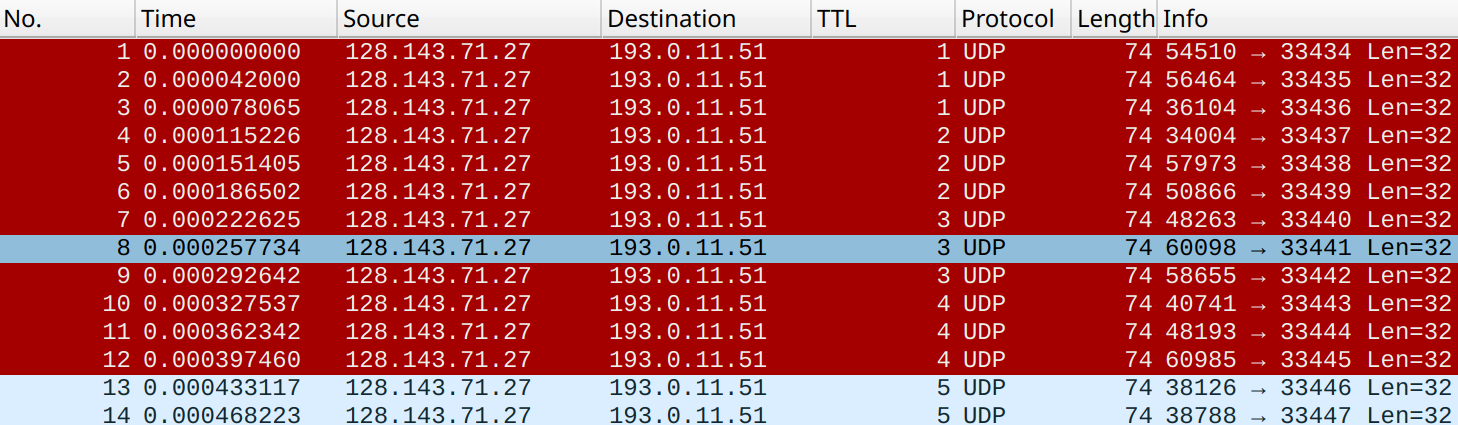
\includegraphics[width=\textwidth]{../routing/traceroute-v4-send}
\end{frame}

\begin{frame}{traceroute received}
% FIXME: screenshot
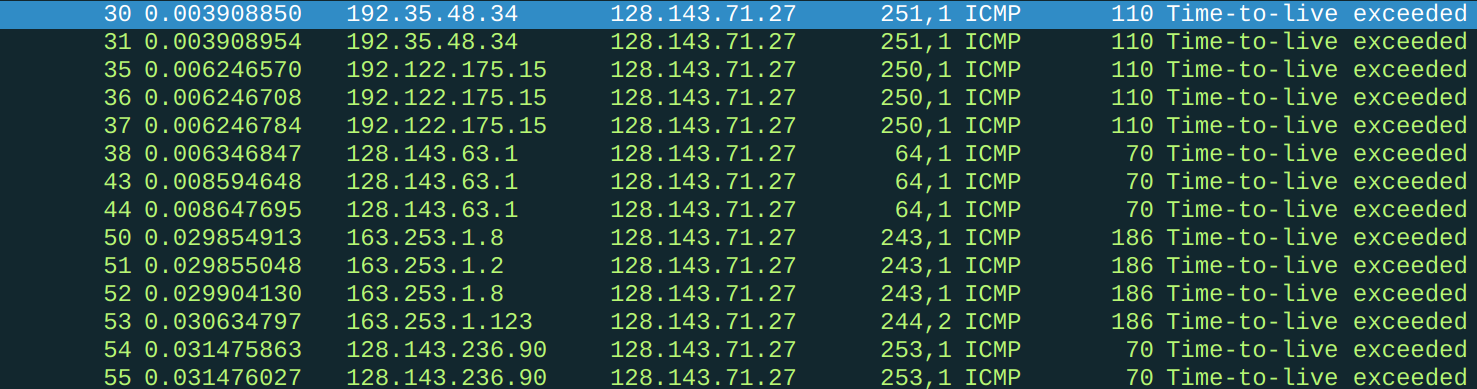
\includegraphics[width=\textwidth]{../routing/traceroute-v4-recv}
\end{frame}

\begin{frame}{aside: multiple paths}
    \begin{itemize}
    \item only showing \textit{forward} path
        \begin{itemize}
        \item routing in reverse direction is often different
        \end{itemize}
    \item sometimes multiple forward paths
        \begin{itemize}
        \item way we've shown routing table so far does not allow this
        \end{itemize}
    \end{itemize}
\end{frame}
